\documentclass[a4paper]{article}
\usepackage[utf8]{inputenc}
\usepackage[russian]{babel}
\usepackage[margin=1in]{geometry}
\usepackage{float}
\usepackage{graphicx}
\usepackage{setspace}
\usepackage{breqn}
\title{Лабораторная работа}
\author{Шулайкин Д.А.}
\begin{document}
\onehalfspacing
\thispagestyle{empty}
\begin{center}
Министерство образования и науки Российской Федерации
\vspace{10pt}

Федеральное государственное бюджетное образовательное учереждение высшего образования учреждения высшего профессионального образования "Ивановский государственный энергетический университет имени В.И. Ленина"
\vspace{40pt}

Кафедра электроники и микропроцессорных систем
\vspace{40pt}

\textbf{Отчет по лабораторной работе №1}

Дисциплина: Схемотехника

Тема: ИССЛЕДОВАНИЕ ЭЛЕМЕНТОВ, УЗЛОВ И УСТРОЙСТВ ЦИФРОВОЙ ВЫЧИСЛИТЕЛЬНОЙ ТЕХНИКИ

\end{center}

\vspace{310pt}
\begin{flushright}
\textbf{Список участников} \\
Шулайкин Д. А. \\
Ужастин К. А. \\

\textbf{Проверил:}
Тарасов С.В.
\end{flushright}
\vspace{40pt}
\begin{center}
Иваново 2018
\end{center}
\pagebreak

\section{План}
\subsection{Рисунок}
\subsection{Таблица истинности}
\subsection{Вывод по таблице истинности}

\section{Схема I-1}
\subsection{Рисунок}
\begin{figure}[H]
    \centering
    \includegraphics[width=300pt]{1.png}
\end{figure}

\subsection{Таблица истинности}
\begin{table}[H]
\centering
\begin{tabular}{|c|c|c|}
\hline
$SA1$ & $SA2$ & $HL1 = D2.1$ \\
\hline
0 & 0 & 1 \\
0 & 1 & 1 \\
1 & 0 & 1 \\
1 & 1 & 0 \\
\hline
\end{tabular}
\end{table}

\subsection{Вывод по таблице истинности}
$D2.1$ - И-НЕ.
\subsubsection{ДНФ}
$$ HL1 = (\neg SA1 * \neg SA2) + (\neg SA1 * SA2) + (SA1 * \neg SA2) $$
\subsubsection{КНФ}
$$ HL1 = \neg SA1 + \neg SA2 $$

\pagebreak

\section{Схема I-2}
\subsection{Рисунок}
\begin{figure}[H]
    \centering
    \includegraphics[width=300pt]{2.png}
\end{figure}
\subsection{Таблица истинности}
\begin{table}[H]
    \centering
    \begin{tabular}{|c|c|c|c|}
        \hline
        $SA1$ & $SA2$ & $D2.2$ & $HL1 = D2.2$\\
        \hline
        0 & 0 & 1 & 0 \\
        0 & 1 & 1 & 0 \\
        1 & 0 & 1 & 0 \\
        1 & 1 & 0 & 1 \\
        \hline
    \end{tabular}
\end{table}

\subsection{Вывод по таблице истинности}
$D2.2$ - НЕ
\subsubsection{ДНФ}
$$ HL1 = SA1 * SA2 $$
\subsubsection{КНФ}
$$ HL1 = (SA1 + SA2) * (SA1 + \neg SA2) * (\neg SA1 + \neg SA2) $$

\pagebreak

\section{Схема I-3}
\subsection{Рисунок}
\begin{figure}[H]
    \centering
    \includegraphics[width=300pt]{3.png}
\end{figure}
\subsection{Таблица истинности}
\begin{table}[ht]
    \centering
    \begin{tabular}{|c|c|c|}
        \hline
        $SA1$ & $SA2$ & $HL1 = D1.1$\\
        \hline
        0 & 0 & 1 \\
        0 & 1 & 0 \\
        1 & 0 & 0 \\
        1 & 1 & 0 \\
        \hline
    \end{tabular}
\end{table}

\subsection{Вывод по таблице истинности}
$D1.1$ - ИЛИ-НЕ
\subsubsection{ДНФ}
$$ HL1 = (\neg SA1 * \neg SA2) $$
\subsubsection{КНФ}
$$ (SA1 + \neg SA2)*(\neg SA1 + SA2)*(\neg SA1 + \neg SA2)$$

\pagebreak

\section{Схема I-4}
\subsection{Рисунок}
\begin{figure}[H]
    \centering
    \includegraphics[width=300pt]{4.png}
\end{figure}
\subsection{Таблица истинности}
\begin{table}[H]
    \centering
    \begin{tabular}{|c|c|c|c|}
        \hline
        $SA1$ & $SA2$ & $D1.1$ & $HL1 = D1.2$\\
        \hline
        0 & 0 & 1 & 0 \\
        0 & 1 & 0 & 1 \\
        1 & 0 & 0 & 1 \\
        1 & 1 & 0 & 1 \\
        \hline
    \end{tabular}
\end{table}

\subsection{Вывод по таблице истинности}
$D1.2$ - НЕ
\subsubsection{ДНФ}
$$ HL1 = (\neg SA1 * SA2) + (SA1 * \neg SA2) + (\neg SA1 * \neg SA2)$$
\subsubsection{КНФ}
$$ HL1 = SA1 + SA2 $$

\pagebreak

\section{Схема I-5}
\subsection{Рисунок}
\begin{figure}[H]
    \centering
    \includegraphics[width=300pt]{5.png}
\end{figure}
\subsection{Таблица истинности}
\begin{table}[H]
    \centering
    \begin{tabular}{|c|c|c|}
        \hline
        $SA1$ & $SA2$ & $HL1 = D3.1$\\
        \hline
        0 & 0 & 0 \\
        0 & 1 & 1 \\
        1 & 0 & 1 \\
        1 & 1 & 0 \\
        \hline
    \end{tabular}
\end{table}

\subsection{Вывод по таблице истинности}
$ D3.1 $ - XOR
\subsubsection{ДНФ}
$$ HL1 = (\neg SA1 * SA2) + (SA1 * \neg SA2)$$
\subsubsection{КНФ}
$$ HL1 = (SA1 + SA2)*(\neg SA1 + \neg SA2)$$

\pagebreak


\section{Схема I-6}
\subsection{Рисунок}
\begin{figure}[H]
    \centering
    \includegraphics[width=300pt]{6.png}
\end{figure}
\subsection{Таблица истинности}
\begin{table}[H]
    \centering
    \begin{tabular}{|c|c|c|c|c|}
        \hline
        $SA1$ & $SA2$ & $D3.1$ & $HL1 = DS2.3$ \\
        \hline
        0 & 0 & 0 & 1 \\
        0 & 1 & 1 & 0 \\
        1 & 0 & 1 & 0 \\
        1 & 1 & 0 & 1 \\
        \hline
    \end{tabular}
\end{table}

\subsection{Вывод по таблице истинности}
$DS2.3$ - НЕ
\subsubsection{ДНФ}
$$ HL1 = (\neg SA1 * \neg SA2) + (SA1 * SA2)$$
\subsubsection{КНФ}
$$ HL1 = (SA1 + \neg SA2) * (\neg SA1 + SA2)$$

\pagebreak


\section{Схема  I-7}
\subsection{Рисунок}
\begin{figure}[H]
    \centering
    \includegraphics[width=300pt]{7.png}
\end{figure}
\subsection{Таблица истинности}
\begin{table}[H]
    \centering
    \begin{tabular}{|c|c|c|c|c|c|}
        \hline
        $SA1$ & $SA2$ & $SA3$ & $DS3.1$ & $HL1 = D3.2$ \\
        \hline
        0 & 0 & 0 & 0 & 0\\
        0 & 0 & 1 & 0 & 1\\
        0 & 1 & 0 & 1 & 1\\
        0 & 1 & 1 & 1 & 0\\
        1 & 0 & 0 & 1 & 1\\
        1 & 0 & 1 & 1 & 0\\
        1 & 1 & 0 & 0 & 0\\
        1 & 1 & 1 & 0 & 1\\
        \hline
    \end{tabular}
\end{table}

\subsection{Вывод по таблице истинности}
$D3.2$ - XOR
$$ HL = (SA1 \oplus SA2) \oplus SA3 $$
\subsubsection{ДНФ}
$$ F = (\neg SA1*\neg SA2*SA3) + (\neg SA1*SA2 \neg SA3) + (\neg SA1*SA2*SA3) + ( SA1*SA2*SA3) $$
\subsubsection{КНФ}
$$ F = (SA1 + SA2 + SA3) * (SA1 + \neg SA2 + \neg SA3) * (\neg SA4 + SA5 + \neg SA6) * ( \neg SA1 + \neg SA2 + SA3 ) $$

\pagebreak


\section{Схема I-8}
\subsection{Рисунок}
\begin{figure}[H]
    \centering
    \includegraphics[width=300pt]{8.png}
\end{figure}
\subsection{Таблица истинности}
\begin{table}[H]
    \centering
    \begin{tabular}{|c|c|c|c|c|c|c|c|}
        \hline
        $SA1$ & $SA2$ & $SA4$ & $SA5$ & $D3.1$ & $D3.2$ & $HL1 = D1.4$\\
        \hline
        0 & 0 & 0 & 0 & 0 & 0 & 1 \\
        0 & 0 & 0 & 1 & 0 & 1 & 0 \\
        0 & 0 & 1 & 0 & 0 & 1 & 0 \\
        0 & 0 & 1 & 1 & 0 & 0 & 1 \\
        0 & 1 & 0 & 0 & 1 & 0 & 0 \\
        0 & 1 & 0 & 1 & 1 & 1 & 0 \\
        0 & 1 & 1 & 0 & 1 & 1 & 0 \\
        0 & 1 & 1 & 1 & 1 & 0 & 0 \\
        1 & 0 & 0 & 0 & 1 & 0 & 0 \\
        1 & 0 & 0 & 1 & 1 & 1 & 0 \\
        1 & 0 & 1 & 0 & 1 & 1 & 0 \\
        1 & 0 & 1 & 1 & 1 & 0 & 0 \\
        1 & 1 & 0 & 0 & 0 & 0 & 1 \\
        1 & 1 & 0 & 1 & 0 & 1 & 0 \\
        1 & 1 & 1 & 0 & 0 & 1 & 0 \\
        1 & 1 & 1 & 1 & 0 & 0 & 1 \\
        \hline
    \end{tabular}
\end{table}
\subsection{Вывод по таблице истинности}
$D1.4$ - ИЛИ-НЕ
% $ HL1 = \neg((SA1 \oplus SA2) + (SA3 \oplus SA5))$  
\subsubsection{ДНФ}
\begin{dmath}
    HL1  = (\neg SA1*\neg SA2 *\neg SA4 *\neg SA5) + (\neg SA1*\neg SA2*SA4*SA5) + (SA1*SA2*\neg SA4*\neg SA5) + ( SA1*SA2* SA4*SA5)
\end{dmath}

\pagebreak

\section{Схема I-9}
\subsection{Рисунок}
\begin{figure}[H]
    \centering
    \includegraphics[width=300pt]{9.png}
\end{figure}
\subsection{Таблица истинности}
\begin{table}[H]
    \centering
    \begin{tabular}{|c|c|c|c|c|c|c|c|}
        \hline
        $SA1$ & $SA2$ & $D1.1$ & $D2.1$ & $HL1 = D1.3$ & $HL2 = D2.2$\\
        \hline
        0 & 0 & 1 & 1 & 0 & 0 \\
        0 & 1 & 0 & 1 & 1 & 0 \\
        1 & 0 & 0 & 1 & 1 & 0 \\
        1 & 1 & 0 & 0 & 0 & 1 \\
        \hline
    \end{tabular}
\end{table}

\subsection{Вывод по таблице истинности}
$D1.3$ - ИЛИ
\subsubsection{ДНФ}
$$ HL1 = (\neg SA1 * SA2) + (SA1 * \neg SA2)$$ 
$$ HL2 = SA1*SA2 $$ 
\subsubsection{КНФ}
$$ HL1 = (SA1 + SA2) * (\neg SA1 + \neg SA2 ) $$
$$ HL2 =  (SA1 + SA2) * (SA1 + \neg SA2) * (\neg SA1 + SA2) $$

\end{document}